\section{\trFatJoin{}、\trFatSlice{}与\trMappingSpace{}}
\label{sec:fat-joins-fat-slices-mapping-spaces}

本节我们将构造\trJoin{}的一个替代品，并证明它\trJoyalEquivalence{}于%
第 1 章中的\cref{def:join-simplicial-sets}所给出的构造，这里仍追随\trRezk{}的讲义 \cite{Rez20}。
这一结果随后将被用来比较∞-\trCategory{}中\trMappingSpace{}的不同模型。我们还将为%
\trIsofibration{}导出若干更有用的提升性质。对于讨论∞-\trCategory{}中的\trLimit{}与%
\trColimit{}，胖联与\trFatSlice{}也将被证明特别有用。本节将以单纯\trCategory{}的%
\trCoherentNerve{}中的\trMappingSpace{}与该单纯\trCategory{}中现成的 hom-单纯集%
（hom-simplicial sets）之间的比较收尾，不过将不给证明。

\begin{definition}\label{def:fat-join}
设 $X$ 与 $Y$ 是\trSimplicialSets{}。我们定义一个新的\trSimplicialSet{} $X \diamond Y$
为\trPushout{}%
\begin{center}
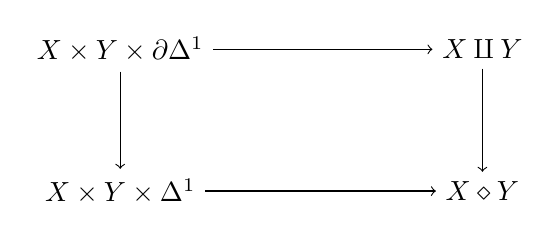
\begin{tikzpicture}
  \node (tl) at (0,0) {$X \times Y \times \partial\Delta^1$};
  \node (tr) at (4.6,0) {$X \amalg Y$};
  \node (bl) at (0,-1.8) {$X \times Y \times \Delta^1$};
  \node (br) at (4.6,-1.8) {$X \diamond Y$};
  \draw[->] (tl) -- (tr);
  \draw[->] (tl) -- (bl);
  \draw[->] (bl) -- (br);
  \draw[->] (tr) -- (br);
\end{tikzpicture}
\end{center}
其中顶上的水平箭头把三元组 $(x, y, 0)$ 送到 $x$，把三元组 $(x, y, 1)$ 送到 $y$。
这个\trSimplicialSet{}称为\emph{\trFatJoin{}}（fat join）。
\end{definition}

\begin{lemma}\label{lem:fat-join-colimit}
对固定的 $Y$，对应 $X \mapsto X \diamond Y$ 可扩充为一个保持余极限的\trFunctor{}%
$\mathrm{sSet} \to \mathrm{sSet}_{Y/}$。对映射 $X \mapsto Y \diamond X$ 亦然。
\end{lemma}

\begin{proof}
第一个断言是一个容易的计算：我们需要验证，对任何\trMorphism{} $X \to X'$，图表
\begin{center}
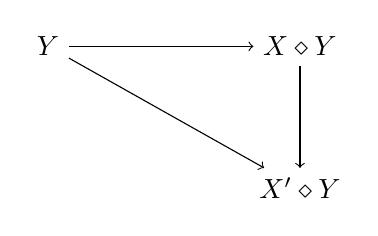
\begin{tikzpicture}
  \node (y) at (0,0) {$Y$};
  \node (xy) at (3.2,0) {$X \diamond Y$};
  \node (xy2) at (3.2,-1.8) {$X' \diamond Y$};
  \draw[->] (y) -- (xy);
  \draw[->] (y) -- (xy2);
  \draw[->] (xy) -- (xy2);
\end{tikzpicture}
\end{center}
交换。但这无非由如下图表交换这一事实得出：
\begin{center}
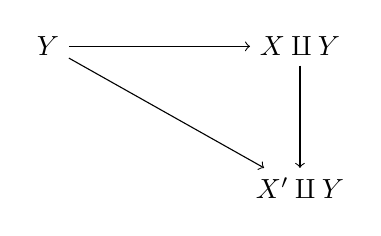
\begin{tikzpicture}
  \node (y) at (0,0) {$Y$};
  \node (xy) at (3.2,0) {$X \amalg Y$};
  \node (xy2) at (3.2,-1.8) {$X' \amalg Y$};
  \draw[->] (y) -- (xy);
  \draw[->] (y) -- (xy2);
  \draw[->] (xy) -- (xy2);
\end{tikzpicture}
\end{center}
为了看出这个\trFunctor{}与余极限交换，又只需证明它与余积以及余等化子交换。
于是设 $X$、$X'$ 与 $Y$ 是\trSimplicialSets{}。我们需要证明图表
\begin{center}
\begin{tikzpicture}
  \node (y) at (0,0) {$Y$};
  \node (xy) at (4.6,0) {$X \diamond Y$};
  \node (x2y) at (0,-1.8) {$X' \diamond Y$};
  \node (push) at (4.6,-1.8) {$(X \amalg X') \diamond Y$};
  \draw[->] (y) -- (xy);
  \draw[->] (y) -- (x2y);
  \draw[->] (x2y) -- (push);
  \draw[->] (xy) -- (push);
\end{tikzpicture}
\end{center}
是单纯集中的\trPushout{}。但这立即可由定义得出。接下来，我们回忆 $\mathrm{sSet}_{Y/}$
中的余等化子是经由遗忘\trFunctor{} $\mathrm{sSet}_{Y/} \to \mathrm{sSet}$ 计算的，
见第 1 章中的\cref{lem:slice-complete}。于是设
\[
X \rightrightarrows X' \longrightarrow C
\]
是一个余等化子图表。我们需要证明：应用 $- \diamond Y$ 之后仍得到一个余等化子图表。
此时\trFunctor{} $- \times Y \times \partial\Delta^1$ 与 $- \times Y \times \Delta^1$
是左伴随，因而保持这个余等化子图表。图表
\[
X \amalg Y \rightrightarrows X' \amalg Y \longrightarrow C \amalg Y
\]
确实是一个余等化子：给定一个映射 $X' \amalg Y \to T$，它与所给两个映射的预复合给出
同一个映射 $X \amalg Y \to T$，我们发现恰如所需地存在唯一的从 $C$ 到 $T$ 的映射以及
从 $Y$ 到 $T$ 的映射。最后，既然两个余极限总可交换，我们可以在余等化子上取推出，
从而得到推出的余等化子。这就证明了本引理。
\end{proof}

\begin{observation}\label{obs:fat-join-projection}
存在一个\trSimplicialSets{}的典范映射 $X \diamond Y \to \Delta^1$，它由交换图表
\begin{center}
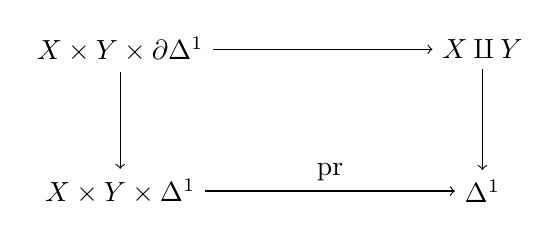
\begin{tikzpicture}
  \node (tl) at (0,0) {$X \times Y \times \partial\Delta^1$};
  \node (tr) at (4.6,0) {$X \amalg Y$};
  \node (bl) at (0,-1.8) {$X \times Y \times \Delta^1$};
  \node (br) at (4.6,-1.8) {$\Delta^1$};
  \draw[->] (tl) -- (tr);
  \draw[->] (tl) -- (bl);
  \draw[->] (bl) -- node[above] {$\mathrm{pr}$} (br);
  \draw[->] (tr) -- (br);
\end{tikzpicture}
\end{center}
所诱导，其中右边的竖直映射由 $X \to \Delta^{\{0\}}$ 与 $Y \to \Delta^{\{1\}}$
组合给出。
\end{observation}

\begin{lemma}\label{lem:fat-join-to-join}
设 $X$ 与 $Y$ 是\trSimplicialSets{}。那么存在一个典范映射 $X \diamond Y \to X \star Y$，
它与到 $\Delta^1$ 的投影以及 $X$ 与 $Y$ 的包含相交换。此映射对 $X$ 与 $Y$ 是函子的。
\end{lemma}

\begin{proof}
回忆第 1 章中的\cref{lem:factorization-over-delta-1}：对\trSimplicialSets{}的每个映射
$p\colon K \to \Delta^1$，存在典范的分解 $K \to K_0 \star K_1 \to \Delta^1$，其中
$K_i = p^{-1}(\{i\})$。把这个结果应用于我们刚才构造的映射 $X \diamond Y \to \Delta^1$，
我们发现 $(X \diamond Y)_0$ 由\trPushout{}%
\begin{center}
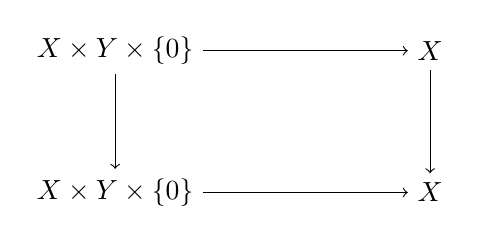
\begin{tikzpicture}
  \node (tl) at (0,0) {$X \times Y \times \{0\}$};
  \node (tr) at (4.0,0) {$X$};
  \node (bl) at (0,-1.8) {$X \times Y \times \{0\}$};
  \node (br) at (4.0,-1.8) {$X$};
  \draw[->] (tl) -- (tr);
  \draw[->] (tl) -- (bl);
  \draw[->] (bl) -- (br);
  \draw[->] (tr) -- (br);
\end{tikzpicture}
\end{center}
给出，并且同样地 $(X \diamond Y)_1$ 由 $Y$ 给出。
\end{proof}

我们接下来将在下述语境中需要\cref{lem:reedy}（\trReedy{} 引理）。

\begin{proposition}\label{prop:pullback-isofibration-joyal-equivalence}
考虑∞-\trCategories{}的一个\trPullback{}图表
\begin{center}
\begin{tikzpicture}
  \node (c) at (0,0) {$\C$};
  \node (d) at (2.6,0) {$\D$};
  \node (c2) at (0,-1.8) {$\C'$};
  \node (d2) at (2.6,-1.8) {$\D'$};
  \draw[->] (c) -- node[above] {$f$} (d);
  \draw[->] (c) -- node[right] {$p'$} (c2);
  \draw[->] (d) -- node[right] {$p$} (d2);
  \draw[->] (c2) -- node[above] {$f'$} (d2);
\end{tikzpicture}
\end{center}
其中映射 $p$ 是一个\trIsofibration{}，而映射 $f'$ 是一个\trJoyalEquivalence{}。
那么映射 $f$ 也是一个\trJoyalEquivalence{}。
\end{proposition}

\begin{proof}
我们将证明：对每个∞-\trCategory{} $\E$，诱导映射
\[
\pi_0\bigl(\mathrm{Fun}(\E, \C)^{\simeq}\bigr) \xrightarrow{\ f_*\ }
\pi_0\bigl(\mathrm{Fun}(\E, \D)^{\simeq}\bigr)
\]
是双射。一旦得证，我们便可取 $\E = \D$，并找到一个\trFunctor{} $g\colon \D \to \C$
使得 $f_*(g) = fg \simeq \mathrm{id}_{\D}$。那时容易看出，$g$ 是 $f$ 的一个逆。

为了证明上面的 $f_*$ 确实是双射，注意图表
\begin{center}
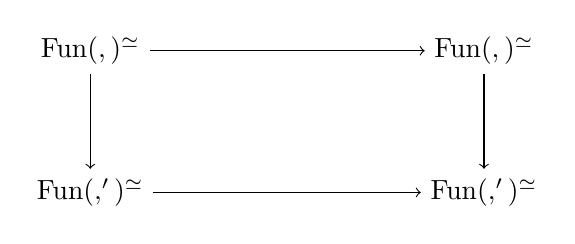
\begin{tikzpicture}
  \node (tl) at (0,0) {$\mathrm{Fun}(\E, \C)^{\simeq}$};
  \node (tr) at (5.0,0) {$\mathrm{Fun}(\E, \D)^{\simeq}$};
  \node (bl) at (0,-1.8) {$\mathrm{Fun}(\E, \C')^{\simeq}$};
  \node (br) at (5.0,-1.8) {$\mathrm{Fun}(\E, \D')^{\simeq}$};
  \draw[->] (tl) -- (tr);
  \draw[->] (tl) -- (bl);
  \draw[->] (tr) -- (br);
  \draw[->] (bl) -- (br);
\end{tikzpicture}
\end{center}
是\trKanComplex{}的一个\trPullback{}图表，其中右边的竖直映射是一个\trKanFibration{}，
而下面的水平映射是一个\trHomotopyEquivalence{}。在\cref{lem:reedy}中我们已经证明，这意味着上面的
水平箭头也是\trHomotopyEquivalence{}，从而特别地在道路分支上诱导一个双射。
\end{proof}

\begin{remark}\label{rem:reedy-explicit}
事实上，在\cref{lem:reedy}的证明中，我们已经明确地证明了：在\trKanComplex{}的%
\trPullback{}图表
\begin{center}
\begin{tikzpicture}
  \node (tl) at (0,0) {$C \times_A B$};
  \node (tr) at (3.2,0) {$B$};
  \node (bl) at (0,-1.8) {$C$};
  \node (br) at (3.2,-1.8) {$A$};
  \draw[->] (tl) -- (tr);
  \draw[->] (tl) -- (bl);
  \draw[->] (tr) -- (br);
  \draw[->] (bl) -- (br);
\end{tikzpicture}
\end{center}
满足映射 $B \to A$ 是一个\trKanFibration{}而映射 $C \to A$ 是一个\trHomotopyEquivalence{}的情形，
诱导映射 $\pi_0(C \times_A B) \to \pi_0(B)$ 是双射——这恰是我们在上述论证中
用到的全部。
\end{remark}

\begin{lemma}\label{lem:pullback-joyal-equivalence}
考虑∞-\trCategories{}的一个图表
\begin{center}
\begin{tikzpicture}
  \node (c) at (0,0) {$\C$};
  \node (d) at (2.6,0) {$\D$};
  \node (e) at (5.2,0) {$\E$};
  \node (c2) at (0,-1.8) {$\C'$};
  \node (d2) at (2.6,-1.8) {$\D'$};
  \node (e2) at (5.2,-1.8) {$\E'$};
  \draw[->, double, double distance=1.2pt] (c) -- (d);
  \draw[->] (e) -- (d);
  \draw[->] (c) -- node[left] {$\simeq$} (c2);
  \draw[->] (d) -- node[left] {$\simeq$} (d2);
  \draw[->] (e) -- node[left] {$\simeq$} (e2);
  \draw[->, double, double distance=1.2pt] (c2) -- (d2);
  \draw[->] (e2) -- (d2);
\end{tikzpicture}
\end{center}
其中诸竖直映射是\trJoyalEquivalence{}，而左边的诸水平映射是\trIsofibration{}。
那么在\trPullback{}上诱导的映射
\[
\C \times_{\D} \E \longrightarrow \C' \times_{\D'} \E'
\]
仍是一个\trJoyalEquivalence{}。
\end{lemma}

\begin{proof}
照搬\cref{lem:pullback-weak-equivalence}的证明，我们同样首先说明如何把证明化归到
两个映射 $\E \to \D$ 与 $\E' \to \D'$ 也是\trIsofibration{}的情形。此处，我们如同%
\cref{lem:localization-factorization}那样把这两个映射函子式地分解为一个作为%
\trJoyalEquivalence{}的\trMonomorphism{}接着一个\trIsofibration{}，于是得到图表
\begin{center}
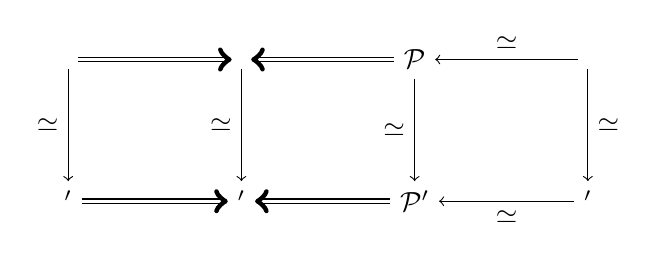
\begin{tikzpicture}
  \node (c) at (0,0) {$\C$};
  \node (d) at (2.2,0) {$\D$};
  \node (p) at (4.4,0) {$\mathcal{P}$};
  \node (e) at (6.6,0) {$\E$};
  \node (c2) at (0,-1.8) {$\C'$};
  \node (d2) at (2.2,-1.8) {$\D'$};
  \node (p2) at (4.4,-1.8) {$\mathcal{P}'$};
  \node (e2) at (6.6,-1.8) {$\E'$};
  \draw[->, double, double distance=1.2pt] (c) -- (d);
  \draw[->, double, double distance=1.2pt] (p) -- (d);
  \draw[->] (e) -- node[above] {$\simeq$} (p);
  \draw[->] (c) -- node[left] {$\simeq$} (c2);
  \draw[->] (d) -- node[left] {$\simeq$} (d2);
  \draw[->] (p) -- node[left] {$\simeq$} (p2);
  \draw[->] (e) -- node[right] {$\simeq$} (e2);
  \draw[->, double, double distance=1.2pt] (c2) -- (d2);
  \draw[->, double, double distance=1.2pt] (p2) -- (d2);
  \draw[->] (e2) -- node[below] {$\simeq$} (p2);
\end{tikzpicture}
\end{center}
其中所有竖直映射都是\trJoyalEquivalence{}。注意，$\mathcal{P}$ 与 $\mathcal{P}'$ 也是∞-\trCategories{}。
于是我们得到一个交换图表
\begin{center}
\begin{tikzpicture}
  \node (tl) at (0,0) {$\C \times_{\D} \E$};
  \node (tr) at (4.6,0) {$\C' \times_{\D'} \E'$};
  \node (bl) at (0,-1.8) {$\C \times_{\D} \mathcal{P}$};
  \node (br) at (4.6,-1.8) {$\C' \times_{\D'} \mathcal{P}'$};
  \draw[->] (tl) -- (tr);
  \draw[->] (tl) -- (bl);
  \draw[->] (tr) -- (br);
  \draw[->] (bl) -- (br);
\end{tikzpicture}
\end{center}
并且我们断言它的诸竖直映射是\trJoyalEquivalence{}：例如，左边的竖直映射出现在
图表
\begin{center}
\begin{tikzpicture}
  \node (a) at (0,0) {$\C \times_{\D} \E$};
  \node (b) at (3.4,0) {$\C \times_{\D} \mathcal{P}$};
  \node (c) at (6.4,0) {$\C$};
  \node (a2) at (0,-1.9) {$\E$};
  \node (b2) at (3.4,-1.9) {$\mathcal{P}$};
  \node (c2) at (6.4,-1.9) {$\D$};
  \draw[->] (a) -- (b);
  \draw[->] (b) -- (c);
  \draw[->] (a) -- (a2);
  \draw[->] (b) -- (b2);
  \draw[->, double, double distance=1.2pt] (c) -- (c2);
  \draw[->] (a2) -- node[above] {$\simeq$} (b2);
  \draw[->] (b2) -- (c2);
\end{tikzpicture}
\end{center}
之中，其中两个正方形都是\trPullback{}。于是我们可以对左边的正方形应用%
\cref{prop:pullback-isofibration-joyal-equivalence}。（对上面右边的竖直映射，
论证相同。）

至此，我们已把证明化归到本引理的陈述之图表中所有水平映射都是\trIsofibration{}%
的情形。

对\cref{prop:pullback-isofibration-joyal-equivalence}作三次应用，如同在%
\cref{lem:pullback-weak-equivalence}中那样考虑所论映射的如下分解，即可完成证明：
\[
\C \times_{\D} \E \longrightarrow (\C' \times_{\D'} \D) \times_{\D} \E
\cong \C' \times_{\D'} \E \longrightarrow \C' \times_{\D'} \E'.
\]
\end{proof}

\begin{corollary}\label{cor:pushout-joyal-equivalence}
设有\trSimplicialSets{}的一个图表
\begin{center}
\begin{tikzpicture}
  \node (x) at (0,0) {$X$};
  \node (y) at (2.6,0) {$Y$};
  \node (z) at (5.2,0) {$Z$};
  \node (x2) at (0,-1.8) {$X'$};
  \node (y2) at (2.6,-1.8) {$Y'$};
  \node (z2) at (5.2,-1.8) {$Z'$};
  \draw[->] (y) -- (x);
  \draw[->] (y) -- (z);
  \draw[->] (x) -- (x2);
  \draw[->] (y) -- (y2);
  \draw[->] (z) -- (z2);
  \draw[->] (y2) -- (x2);
  \draw[->] (y2) -- (z2);
\end{tikzpicture}
\end{center}
其中所有竖直映射是\trJoyalEquivalence{}，而左边的诸水平映射是\trMonomorphism{}。
那么诱导的映射
\[
X \amalg_{Y} Z \longrightarrow X' \amalg_{Y'} Z'
\]
仍是一个\trJoyalEquivalence{}。
\end{corollary}

\begin{proof}
设 $\C$ 是一个∞-\trCategory{}。按定义，我们需要证明映射
\[
\mathrm{Fun}(X' \amalg_{Y'} Z', \C) \longrightarrow \mathrm{Fun}(X \amalg_{Y} Z, \C)
\]
是一个\trJoyalEquivalence{}。但这个映射同构于映射
\[
\mathrm{Fun}(X', \C) \times_{\mathrm{Fun}(Y', \C)} \mathrm{Fun}(Z', \C)
\longrightarrow
\mathrm{Fun}(X, \C) \times_{\mathrm{Fun}(Y, \C)} \mathrm{Fun}(Z, \C),
\]
而由\cref{lem:pullback-joyal-equivalence}与诸假设，后者是一个\trJoyalEquivalence{}。
\end{proof}

\begin{corollary}\label{cor:pushout-product-j}
对所有\trMonomorphism{} $A \to B$，\trPushoutProduct{}映射
\[
J \times A \amalg_{\{0\} \times A} \{0\} \times B \longrightarrow J \times B
\]
是一个\trJoyalEquivalence{}。
\end{corollary}

\begin{proof}
我们考虑如下图表：
\begin{center}
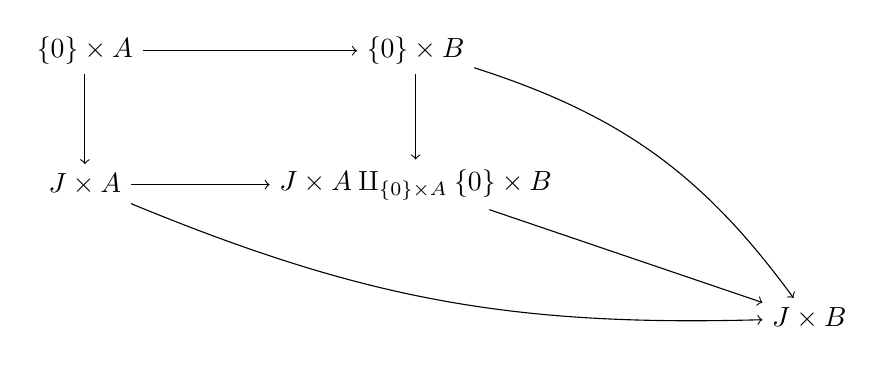
\begin{tikzpicture}
  \node (ta) at (0,0) {$\{0\} \times A$};
  \node (tb) at (4.2,0) {$\{0\} \times B$};
  \node (ma) at (0,-1.7) {$J \times A$};
  \node (mb) at (4.2,-1.7) {$J \times A \amalg_{\{0\} \times A} \{0\} \times B$};
  \node (rb) at (9.2,-3.4) {$J \times B$};
  \draw[->] (ta) -- (tb);
  \draw[->] (ta) -- (ma);
  \draw[->] (tb) -- (mb);
  \draw[->] (ma) -- (mb);
  \draw[->] (mb) -- (rb);
  \draw[->] (tb) to[bend left=18] (rb);
  \draw[->] (ma) to[bend right=12] (rb);
\end{tikzpicture}
\end{center}
诸水平箭头都是\trMonomorphism{}，而左边的竖直箭头与右边那条弯折的箭头都是%
\trJoyalEquivalence{}：这是因为 $\{0\} \to J$ 是\trJoyalEquivalence{}，且正如%
\cref{ex:joyal-equivalence-coproduct-product} 所证，\trJoyalEquivalence{}在有限乘积下封闭。由%
\cref{cor:pushout-joyal-equivalence}，右边的竖直映射也是\trJoyalEquivalence{}；
于是本推论由\trJoyalEquivalence{}的\trThreeForTwoProperty{}得出。
\end{proof}

\begin{definition}\label{def:j-anodyne}
一个\trSimplicialSets{}的映射称为\emph{$J$-\trAnodyne{}}（$J$-anodyne），如果它属于
由\trInnerAnodyne{}映射以及诸形如
$J \times A \amalg_{\{0\} \times A} \{0\} \times B \longrightarrow J \times B$
（其中 $A \to B$ 是\trMonomorphism{}）的映射所生成的\trSaturatedSet{}。
\end{definition}

\begin{corollary}\label{cor:j-anodyne-joyal-equivalence}
每个 $J$-\trAnodyne{}映射都是\trJoyalEquivalence{}。
\end{corollary}

\begin{proof}
我们断言：那些同时又是\trJoyalEquivalence{}的\trMonomorphism{}构成一个%
\trSaturatedSet{}，其证明留作\cref{ex:joyal-equivalence-retract-saturated}。于是只需注意\trInnerAnodyne{}映射是%
\trJoyalEquivalence{}（由\cref{cor:inner-anodyne-joyal-equivalence}），并且形如
$J \times A \amalg_{\{0\} \times A} \{0\} \times B \longrightarrow J \times B$
的映射也是\trJoyalEquivalence{}（由\cref{cor:pushout-product-j}）。
\end{proof}

接下来，我们可以利用\cref{cor:j-anodyne-joyal-equivalence}为 $J$-\trAnodyne{}映射
提供一个更小的生成集，其中所有定义域都是有限\trSimplicialSets{}。这将帮助我们在
本书所呈现的形式下应用\trSmallObjectArgument{}，因为它需要这条技术性假设。

\begin{proposition}\label{prop:j-anodyne-generated}
$J$-\trAnodyne{}映射之集是包含\trInnerAnodyne{}映射与映射 $\{0\} \to J$ 的最小%
\trSaturatedSet{}。
\end{proposition}

\begin{proof}
为记号上的方便，让我们把包含\trInnerAnodyne{}映射与映射 $\{0\} \to J$ 的最小%
\trSaturatedSet{}称为\emph{超 $J$-\trAnodyne{}}（super-$J$-anodyne）映射之集。
显然，超 $J$-\trAnodyne{}映射都是 $J$-\trAnodyne{}映射，于是只需证明：对所有%
\trMonomorphism{} $A \to B$，\trPushoutProduct{}映射
\[
\{0\} \times B \amalg_{\{0\} \times A} J \times A \longrightarrow J \times B
\]
是超 $J$-\trAnodyne{}的。使此情形成立的那些\trMonomorphism{} $A \to B$ 之集本身是
饱和的，因此只需对该断言在 $A \to B$ 为边界包含 $\partial\Delta^n \to \Delta^n$
（$n \ge 0$）的情形加以证明。为此，我们对超 $J$-\trAnodyne{}映射之集使用%
\trSmallObjectArgument{}，便得到我们所感兴趣的映射的如下分解：
\[
\{0\} \times \Delta^n \amalg_{\{0\} \times \partial\Delta^n}
J \times \partial\Delta^n
\xrightarrow{\ i\ } \C \xrightarrow{\ p\ } J \times \Delta^n,
\]
其中 $i$ 是超 $J$-\trAnodyne{}的，而第二个映射对内\trHornInclusion{}与
$\{0\} \to J$ 满足\trRightLiftingProperty{}。由于 $J \times \Delta^n$ 是一个%
∞-\trCategory{}，我们可以推出映射 $\C \to J \times \Delta^n$ 是∞-\trCategories{}%
之间的一个\trIsofibration{}。由于 $J$-\trAnodyne{}映射由\cref{cor:j-anodyne-joyal-equivalence}
是\trJoyalEquivalence{}，而超 $J$-\trAnodyne{}映射是 $J$-\trAnodyne{}的，我们发现
映射 $\C \to J \times \Delta^n$ 实际上是一个\trTrivialFibration{}，从而对提升问题
\begin{center}
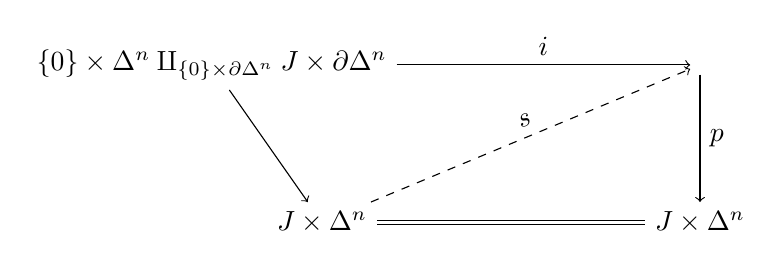
\begin{tikzpicture}
  \node (tl) at (0,0) {$\{0\} \times \Delta^n \amalg_{\{0\} \times \partial\Delta^n} J \times \partial\Delta^n$};
  \node (tr) at (6.2,0) {$\C$};
  \node (bl) at (1.4,-2.0) {$J \times \Delta^n$};
  \node (br) at (6.2,-2.0) {$J \times \Delta^n$};
  \draw[->] (tl) -- node[above] {$i$} (tr);
  \draw[->] (tl) -- (bl);
  \draw[double, double distance=1.2pt] (bl) -- (br);
  \draw[->] (tr) -- node[right] {$p$} (br);
  \draw[->, dashed] (bl) -- node[above, sloped] {$s$} (tr);
\end{tikzpicture}
\end{center}
容有解 $s\colon J \times \Delta^n \to \C$。

考虑图表
\begin{center}
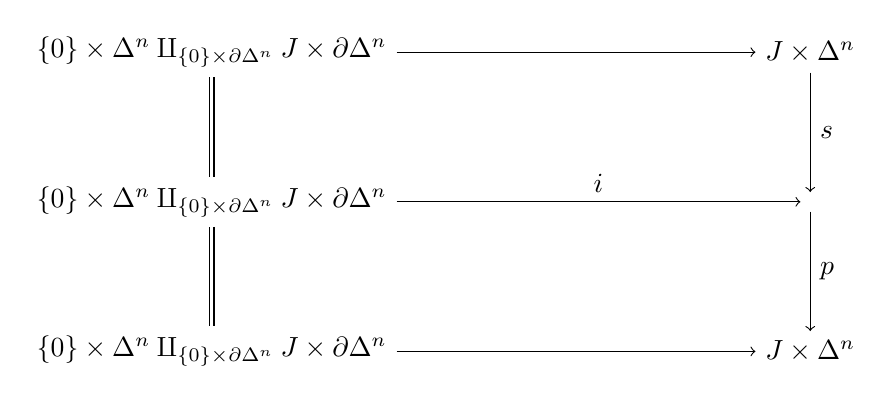
\begin{tikzpicture}
  \node (r1l) at (0,0)
    {$\{0\} \times \Delta^n \amalg_{\{0\} \times \partial\Delta^n} J \times \partial\Delta^n$};
  \node (r1r) at (7.6,0) {$J \times \Delta^n$};
  \node (r2l) at (0,-1.9)
    {$\{0\} \times \Delta^n \amalg_{\{0\} \times \partial\Delta^n} J \times \partial\Delta^n$};
  \node (r2r) at (7.6,-1.9) {$\C$};
  \node (r3l) at (0,-3.8)
    {$\{0\} \times \Delta^n \amalg_{\{0\} \times \partial\Delta^n} J \times \partial\Delta^n$};
  \node (r3r) at (7.6,-3.8) {$J \times \Delta^n$};
  \draw[->] (r1l) -- (r1r);
  \draw[double, double distance=1.2pt] (r1l) -- (r2l);
  \draw[->] (r2l) -- node[above] {$i$} (r2r);
  \draw[double, double distance=1.2pt] (r2l) -- (r3l);
  \draw[->] (r3l) -- (r3r);
  \draw[->] (r1r) -- node[right] {$s$} (r2r);
  \draw[->] (r2r) -- node[right] {$p$} (r3r);
\end{tikzpicture}
\end{center}
我们发现，所感兴趣的映射是超 $J$-\trAnodyne{}映射 $i$ 的一个\trRetract{}，从而它
本身是超 $J$-\trAnodyne{}的。
\end{proof}

若一个\trMonomorphism{}的靶是一个∞-\trCategory{}，那么我们可以证明%
\cref{cor:j-anodyne-joyal-equivalence}的如下更强的版本。

\begin{proposition}\label{prop:j-anodyne-iff-joyal-equivalence}
设 $i\colon A \to B$ 是一个\trMonomorphism{}，其中 $B$ 是一个∞-\trCategory{}。
那么 $i$ 是 $J$-\trAnodyne{}的，当且仅当 $i$ 是一个\trJoyalEquivalence{}。
\end{proposition}

\begin{proof}
由\cref{cor:j-anodyne-joyal-equivalence}，只需证明「若」部分。为此，我们应用%
\trSmallObjectArgument{}，把映射 $A \to B$ 分解为一个复合
\[
A \longrightarrow B' \longrightarrow B,
\]
其中映射 $A \to B'$ 是 $J$-\trAnodyne{}的，而映射 $B' \to B$ 对 $J$-\trAnodyne{}映射
满足\trRightLiftingProperty{}。由于 $B$ 是一个∞-\trCategory{}，这对 $B'$ 同样成立，
且映射 $B' \to B$ 是一个\trIsofibration{}。由\cref{cor:j-anodyne-joyal-equivalence}
与\trJoyalEquivalence{}的\trThreeForTwoProperty{}，映射 $B' \to B$ 是一个%
\trIsofibration{}和一个\trJoyalEquivalence{}，从而由%
\cref{lem:trivial-fibration-joyal-isofibration}是一个\trTrivialFibration{}。%
\footnote{译注：原书此处作「若亚尔纤维化的三取二性质」（the 3-for-2
property for Joyal fibrations），其中「若亚尔纤维化」应为「若亚尔等价」。}选取提升
问题
\begin{center}
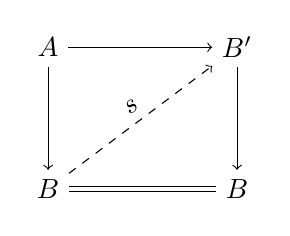
\begin{tikzpicture}
  \node (tl) at (0,0) {$A$};
  \node (tr) at (2.4,0) {$B'$};
  \node (bl) at (0,-1.8) {$B$};
  \node (br) at (2.4,-1.8) {$B$};
  \draw[->] (tl) -- (tr);
  \draw[->] (tl) -- (bl);
  \draw[double, double distance=1.2pt] (bl) -- (br);
  \draw[->] (tr) -- (br);
  \draw[->, dashed] (bl) -- node[above, sloped] {$s$} (tr);
\end{tikzpicture}
\end{center}
的一个解 $s\colon B \to B'$，如同\cref{prop:j-anodyne-generated}的证明中那样，
我们发现映射 $A \to B$ 是 $J$-\trAnodyne{}映射 $A \to B'$ 的一个\trRetract{}，
从而它本身是 $J$-\trAnodyne{}的。
\end{proof}

在本书稍后的阶段（当我们证明对应 $x \mapsto \mathrm{map}_{\C}(x, -)$ 本身对 $x$
是函子的时，以及在第 1 章中的\cref{thm:slice-fibration}关于\trFatSlice{}的类似物中），我们将需要
下述定理。感谢\trNguyen{}对所需化归步骤的解释！

\begin{theorem}\label{thm:isofibration-lifting-joyal-equivalence}
设 $p\colon \C \to \D$ 是∞-\trCategories{}之间的一个\trIsofibration{}，并设
$A \to B$ 是一个同时又是\trJoyalEquivalence{}的\trMonomorphism{}。那么任何提升
问题
\begin{center}
\begin{tikzpicture}
  \node (tl) at (0,0) {$A$};
  \node (tr) at (2.4,0) {$\C$};
  \node (bl) at (0,-1.8) {$B$};
  \node (br) at (2.4,-1.8) {$\D$};
  \draw[->] (tl) -- (tr);
  \draw[->] (tl) -- (bl);
  \draw[->] (bl) -- (br);
  \draw[->] (tr) -- node[right] {$p$} (br);
  \draw[->, dashed] (bl) -- (tr);
\end{tikzpicture}
\end{center}
都容有一个如图中虚箭头所示的解。
\end{theorem}

\begin{proof}
利用\trSmallObjectArgument{}，我们可以把映射 $B \to \D$ 分解为一个 $J$-\trAnodyne{}%
映射 $B \to \mathcal{B}$ 接着一个对 $J$-\trAnodyne{}映射满足\trRightLiftingProperty{}%
的映射 $\mathcal{B} \to \D$。由此可知 $\mathcal{B}$ 是一个∞-\trCategory{}。由于
$J$-\trAnodyne{}映射是\trJoyalEquivalence{}，我们发现复合 $A \to \mathcal{B}$ 是一个%
\trMonomorphism{}和一个\trJoyalEquivalence{}。由%
\cref{prop:j-anodyne-iff-joyal-equivalence}，这个映射是 $J$-\trAnodyne{}的。由于
∞-\trCategories{}之间的\trIsofibration{}对 $J$-\trAnodyne{}映射满足%
\trRightLiftingProperty{}，我们可以在图表
\begin{center}
\begin{tikzpicture}
  \node (a) at (0,0) {$A$};
  \node (c) at (2.4,0) {$\C$};
  \node (b) at (0,-1.8) {$B$};
  \node (b2) at (0,-3.6) {$\mathcal{B}$};
  \node (d) at (2.4,-3.6) {$\D$};
  \draw[->] (a) -- (c);
  \draw[->] (a) -- (b);
  \draw[->] (b) -- (b2);
  \draw[->] (b2) -- (d);
  \draw[->] (c) -- (d);
  \draw[->, dashed] (b2) -- (c);
\end{tikzpicture}
\end{center}
中找到一条虚箭头，它同时也解决原来的提升问题。
\end{proof}

让我们以关于内零调映射的一个漂亮事实来结束这段关于 $J$-\trAnodyne{}映射的插段。
下述引理取自\trStevenson{}（Daniel Stevenson） \cite[Lemma 2.19]{Ste18a}。

\begin{lemma}\label{lem:mono-bijection-inner-anodyne}
设 $\C$ 是一个∞-\trCategory{}，并设 $i\colon A \to \C$ 是一个在 $0$-\trSimplex{}上
为双射的\trMonomorphism{}，同时也是一个\trJoyalEquivalence{}。那么 $i$ 是%
\trInnerAnodyne{}的。
\end{lemma}

\begin{proof}
由\trSmallObjectArgument{}，我们可以把这个映射分解为复合
$A \xrightarrow{\ j\ } \mathcal{B} \xrightarrow{\ p\ } \C$，其中 $j$ 是一个%
\trInnerAnodyne{}映射，而 $p$ 是一个\trInnerFibration{}。由于 $\C$ 是一个%
∞-\trCategory{}，$p$ 满足\cref{ex:inner-fibration-trivial} 的诸假设，因而是一个\trTrivialFibration{}。
如同\cref{prop:j-anodyne-iff-joyal-equivalence}的证明中那样，这表明 $i$ 是 $j$ 的
一个\trRetract{}，从而也是\trInnerAnodyne{}的。
\end{proof}

\begin{corollary}\label{cor:pushout-product-j-inner-anodyne}
设 $K \to L$ 是一个在 $0$-\trSimplex{}上为双射的\trMonomorphism{}。那么映射
\[
\{0\} \times L \amalg_{\{0\} \times K} J \times K \longrightarrow J \times L
\]
是\trInnerAnodyne{}的。
\end{corollary}

\begin{proof}
只需对 $n \ge 1$ 的映射 $\partial\Delta^n \to \Delta^n$ 证明该断言。由构造，这个
映射在 $0$-\trSimplex{}上为双射，由\cref{cor:pushout-product-j}是一个%
\trJoyalEquivalence{}，并且以一个∞-\trCategory{}为靶，因为 $\Delta^n$ 与 $J$ 都是
∞-\trCategories{}。应用\cref{lem:mono-bijection-inner-anodyne}即可完成本推论。
\end{proof}

现在我们回到胖联的重要性质，以及它与 1.4 节中通常\trJoin{}的关系。

\begin{corollary}\label{cor:fat-join-joyal-equivalence}
设 $X \to X'$ 是\trSimplicialSets{}之间的一个\trJoyalEquivalence{}，并设 $Y$ 是一个%
\trSimplicialSet{}。那么映射 $X \diamond Y \to X' \diamond Y$ 是一个%
\trJoyalEquivalence{}。同样地，映射 $Y \diamond X \to Y \diamond X'$ 是一个%
\trJoyalEquivalence{}。
\end{corollary}

\begin{proof}
由于 $X \diamond Y$ 是\trPushout{}%
\begin{center}
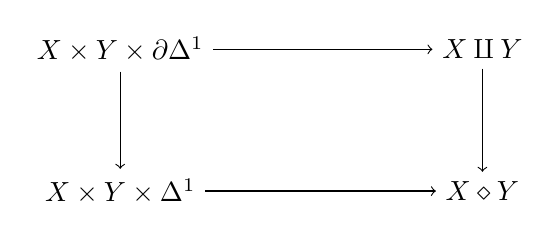
\begin{tikzpicture}
  \node (tl) at (0,0) {$X \times Y \times \partial\Delta^1$};
  \node (tr) at (4.6,0) {$X \amalg Y$};
  \node (bl) at (0,-1.8) {$X \times Y \times \Delta^1$};
  \node (br) at (4.6,-1.8) {$X \diamond Y$};
  \draw[->] (tl) -- (tr);
  \draw[->] (tl) -- (bl);
  \draw[->] (bl) -- (br);
  \draw[->] (tr) -- (br);
\end{tikzpicture}
\end{center}
其中左边的竖直映射是一个\trMonomorphism{}，由\cref{cor:pushout-joyal-equivalence}，
只需证明由 $X \to X'$ 在其余三个角上诱导的映射都是\trJoyalEquivalence{}。但这由%
\cref{ex:joyal-equivalence-coproduct-product} 得出。
\end{proof}

\begin{definition}\label{def:pre-inverse}
一个\trSimplicialSets{}的映射 $f\colon X \to Y$ 称为容有一个\emph{预逆}
（pre-inverse），如果存在映射 $g\colon Y \to X$、
$\tau\colon \Delta^1 \to \mathrm{Hom}(X, X)$ 与
$\tau'\colon \Delta^1 \to \mathrm{Hom}(Y, Y)$，使得
\begin{enumerate}[label=(\arabic*)]
  \item $\tau_\varepsilon = \mathrm{id}_X$ 且 $\tau_{1+\varepsilon} = gf$，其中
        $\varepsilon \in \{0, 1\} \cong \Z/2$；
  \item $\tau'_\varepsilon = \mathrm{id}_Y$ 且 $\tau'_{1+\varepsilon} = fg$，其中
        $\varepsilon$ 同样取自 $\{0, 1\} \cong \Z/2$；
  \item 对 $X$ 的所有\trObject{} $x$，\trMorphism{}%
        $\tau(x)\colon \Delta^1 \to X$ 表示 $X$ 的一条退化边，而对 $Y$ 的所有%
        \trObject{} $y$，$\tau'(y)\colon \Delta^1 \to Y$ 表示 $Y$ 的一条退化边。
\end{enumerate}
\end{definition}

\begin{proposition}\label{prop:fat-join-joyal-equivalence}
设 $X$ 与 $Y$ 是\trSimplicialSets{}。那么\cref{lem:fat-join-to-join}的典范映射
$X \diamond Y \to X \star Y$ 是一个\trJoyalEquivalence{}。
\end{proposition}

\begin{proof}
如\cref{lem:fat-join-colimit}与第 1 章中的\cref{lem:join-preserves-colimits}中所注意到的，
\trFunctor{} $- \diamond Y$ 与 $- \star Y$ 二者都与\trFiltered{}余极限交换。此外，
若把它们视为取值于 $\mathrm{sSet}_{Y/}$ 中，则二者都与余积交换。于是我们可以把一般
情形化归到 $X$ 只有有限多个非退化\trSimplex{}而且\trConnected{}的情形。在这种情形
下，我们可以把 $X$ 写成\trPushout{} $X' \amalg_{\partial\Delta^n} \Delta^n$。由于
推出是连通余极限，我们也得到同构
\[
X \diamond Y \cong X' \diamond Y \amalg_{\partial\Delta^n \diamond Y} \Delta^n \diamond Y
\]
以及在把 $\diamond$ 换成 $\star$ 时的类似同构。于是只需对 $X'$、$\partial\Delta^n$
与 $\Delta^n$ 证明该断言。由相同的推理，对 $\Delta^n$（对所有 $n$）的陈述经由归纳
蕴含对 $\partial\Delta^n$ 与 $X'$ 的陈述。因此，剩下要证明的是
\[
\Delta^n \diamond Y \longrightarrow \Delta^n \star Y
\]
是一个\trJoyalEquivalence{}。现在，包含 $I^n \to \Delta^n$ 由第 1 章中的%
\cref{prop:spine-inner-anodyne}是\trInnerAnodyne{}的，于是在图表
\begin{center}
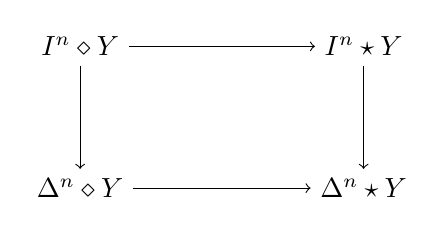
\begin{tikzpicture}
  \node (tl) at (0,0) {$I^n \diamond Y$};
  \node (tr) at (3.6,0) {$I^n \star Y$};
  \node (bl) at (0,-1.8) {$\Delta^n \diamond Y$};
  \node (br) at (3.6,-1.8) {$\Delta^n \star Y$};
  \draw[->] (tl) -- (tr);
  \draw[->] (tl) -- (bl);
  \draw[->] (tr) -- (br);
  \draw[->] (bl) -- (br);
\end{tikzpicture}
\end{center}
中，两个竖直映射都是\trJoyalEquivalence{}：对左边的竖直映射，这是%
\cref{cor:fat-join-joyal-equivalence}；而对右边的竖直映射，这是 $- \star Y$ 保持%
\trInnerAnodyne{}映射这一事实，见第 1 章中的\cref{lem:join-box-anodyne}的（1）。（实际上，它
甚至把\trRightAnodyne{}映射送到\trInnerAnodyne{}映射。）因此，只需对 $I^n$ 证明该
陈述。由于 $I^n \cong I^{n-1} \amalg_{\Delta^0} \Delta^1$，最终只需处理 $X$ 为
$\Delta^0$ 或 $\Delta^1$ 的情形。现在我们观察到 $\Delta^0$ 是 $\Delta^1$ 的一个%
\trRetract{}，因此映射
\[
\Delta^0 \diamond Y \longrightarrow \Delta^0 \star Y
\]
是映射
\[
\Delta^1 \diamond Y \longrightarrow \Delta^1 \star Y
\]
的一个\trRetract{}。由于\trJoyalEquivalence{}的\trRetract{}是\trJoyalEquivalence{}%
（见\cref{ex:joyal-equivalence-retract-saturated}），只需证明后者对所有的 $Y$ 都是\trJoyalEquivalence{}。对 $Y$ 执行同样
的化归，最终只需证明映射
\[
\Delta^1 \diamond \Delta^1 \to \Delta^1 \star \Delta^1 \cong \Delta^3
\]
是一个\trJoyalEquivalence{}。为此，我们将（几乎）为这个映射构造一个\emph{预逆}
（pre-inverse）。实际上，我们将构造一串由此类预逆组成的之字形（zig-zag），把恒等
与一个待构造的逆连接起来。为了构造这个映射，我们首先从定义观察到，存在典范的商映射
$(\Delta^1)^{\times 3} \to \Delta^1 \diamond \Delta^1$。我们断言复合
\[
\mathrm{can}\colon (\Delta^1)^{\times 3} \longrightarrow \Delta^1 \diamond \Delta^1
\longrightarrow \Delta^3
\]
由公式
\[
(a, b, c) =
\begin{cases}
a & \text{若 } c = 0, \\
b + 2 & \text{若 } c = 1.
\end{cases}
\]
给出。这只是对定义的一个显式验证。然后我们考虑 $(\Delta^1)^{\times 3}$ 的由
\[
(000) \longrightarrow (100) \longrightarrow (101) \longrightarrow (111)
\]
所表示的 $3$-\trSimplex{} $\sigma$ 及其在 $\Delta^1 \diamond \Delta^1$ 中的像。
首先，我们观察到复合
\[
\Delta^3 \longrightarrow \Delta^1 \diamond \Delta^1 \longrightarrow \Delta^3
\]
是恒等。

然后我们必须构造一个映射
$\Delta^1 \to \mathrm{Hom}(\Delta^1 \diamond \Delta^1,\, \Delta^1 \diamond \Delta^1)$，
它把映射 $\sigma$ 展示为典范映射 $\Delta^1 \diamond \Delta^1 \to \Delta^3$ 的预逆。
我们将分三步来做这件事：首先，我们将构造两个映射
$\Delta^1 \to \mathrm{Hom}((\Delta^1)^{\times 3},\, (\Delta^1)^{\times 3})$，把恒等
连接到一个辅助映射 $\Phi$，再把 $\Phi$ 连接到 $\sigma \circ \mathrm{can}$；其次，
我们将证明它们下降为 $\Delta^1 \diamond \Delta^1$ 之间的映射；最后，我们将证明两个
所得映射都具有如下性质：对固定的\trObject{}，$\Delta^1 \diamond \Delta^1$ 中所诱导
的边是一条退化边。

在下面的图中，左边的立方体表示 $(\Delta^1)^3$ 的恒等，中间的立方体表示映射 $\Phi$，
而右边的立方体表示复合 $\sigma \circ \mathrm{can}$。注意，从中间的立方体到两个外侧
立方体都存在显而易见的映射。

\begin{center}
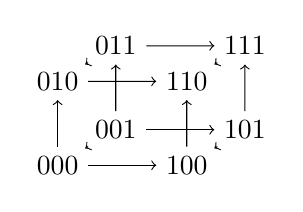
\begin{tikzpicture}[scale=0.82]
  \node (A) at (0,0) {$000$};
  \node (B) at (2,0) {$100$};
  \node (C) at (0.9,0.55) {$001$};
  \node (D) at (2.9,0.55) {$101$};
  \node (E) at (0,1.3) {$010$};
  \node (F) at (2,1.3) {$110$};
  \node (G) at (0.9,1.85) {$011$};
  \node (H) at (2.9,1.85) {$111$};
  \draw[->] (A) -- (B);
  \draw[->] (C) -- (D);
  \draw[->] (E) -- (F);
  \draw[->] (G) -- (H);
  \draw[->] (A) -- (E);
  \draw[->] (B) -- (F);
  \draw[->] (C) -- (G);
  \draw[->] (D) -- (H);
  \draw[->] (A) -- (C);
  \draw[->] (B) -- (D);
  \draw[->] (E) -- (G);
  \draw[->] (F) -- (H);
\end{tikzpicture}
\hspace{0.9cm}
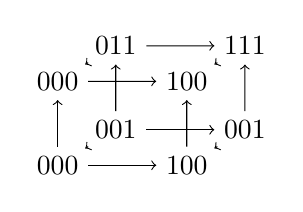
\begin{tikzpicture}[scale=0.82]
  \node (A) at (0,0) {$000$};
  \node (B) at (2,0) {$100$};
  \node (C) at (0.9,0.55) {$001$};
  \node (D) at (2.9,0.55) {$001$};
  \node (E) at (0,1.3) {$000$};
  \node (F) at (2,1.3) {$100$};
  \node (G) at (0.9,1.85) {$011$};
  \node (H) at (2.9,1.85) {$111$};
  \draw[->] (A) -- (B);
  \draw[->] (C) -- (D);
  \draw[->] (E) -- (F);
  \draw[->] (G) -- (H);
  \draw[->] (A) -- (E);
  \draw[->] (B) -- (F);
  \draw[->] (C) -- (G);
  \draw[->] (D) -- (H);
  \draw[->] (A) -- (C);
  \draw[->] (B) -- (D);
  \draw[->] (E) -- (G);
  \draw[->] (F) -- (H);
\end{tikzpicture}
\hspace{0.9cm}
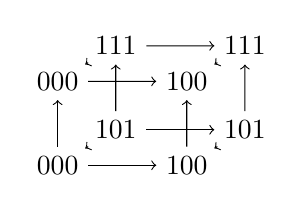
\begin{tikzpicture}[scale=0.82]
  \node (A) at (0,0) {$000$};
  \node (B) at (2,0) {$100$};
  \node (C) at (0.9,0.55) {$101$};
  \node (D) at (2.9,0.55) {$101$};
  \node (E) at (0,1.3) {$000$};
  \node (F) at (2,1.3) {$100$};
  \node (G) at (0.9,1.85) {$111$};
  \node (H) at (2.9,1.85) {$111$};
  \draw[->] (A) -- (B);
  \draw[->] (C) -- (D);
  \draw[->] (E) -- (F);
  \draw[->] (G) -- (H);
  \draw[->] (A) -- (E);
  \draw[->] (B) -- (F);
  \draw[->] (C) -- (G);
  \draw[->] (D) -- (H);
  \draw[->] (A) -- (C);
  \draw[->] (B) -- (D);
  \draw[->] (E) -- (G);
  \draw[->] (F) -- (H);
\end{tikzpicture}
\end{center}

现在需要验证：这些映射在与投影作后复合（post-composition）之后，下降到商
$\Delta^1 \diamond \Delta^1$。
为此，我们首先观察到，所有这些立方体都限制为
$\Delta^1 \times \Delta^1 \times \partial\Delta^1$ 的自同态。更具体地说，这意味着：如果只看前层与后层（也就是说，
忽略对角映射）并投影到第三个坐标，那么只剩下恒等\trMorphism{}。接下来，我们发现
$\Delta^1 \amalg \Delta^1$ 存在相容的自同态，因为 $\Delta^1 \amalg \Delta^1$ 的恒等
对 $\Phi$ 与 $\sigma \circ \mathrm{can}$ 二者都是相容的。这表明 $\Phi$ 与
$\sigma \circ \mathrm{can}$ 下降到推出 $\Delta^1 \diamond \Delta^1$。

或者，可以看出 $\Delta^1 \diamond \Delta^1$ 是 $(\Delta^1)^{\times 3}$ 的商，其中子%
\trSimplicialSet{} $\Delta^1 \times \Delta^1 \times \{0\}$ 被（经由第一个投影）坍缩
为 $\Delta^1$，而子\trSimplicialSet{} $\Delta^1 \times \Delta^1 \times \{1\}$ 被
（经由第二个投影）坍缩为 $\Delta^1$。于是我们必须检验：$\Phi$ 与
$\sigma \circ \mathrm{can}$ 在随后施加这个投影之后是否在适当的意义下不变，也就是说，$F(x, y, 0)$ 是否不依赖
于 $y$，而 $F(x, y, 1)$ 是否不依赖于 $x$。但这只是一个显式的验证。

接下来，我们观察到：$\Delta^1 \times \Delta^1 \times \partial\Delta^1$ 中任何被映为
$\Delta^1 \amalg \Delta^1$ 的一个恒等（即一条退化边）的\trMorphism{}，也被映为
$\Delta^1 \diamond \Delta^1$ 中的一条退化边。这表明，从中间的立方体到左边与右边的
立方体的所有映射都是 $\Delta^1 \diamond \Delta^1$ 中的退化边；这蕴含立方体之间的诸
水平映射也下降为
$\mathrm{Hom}(\Delta^1 \diamond \Delta^1,\, \Delta^1 \diamond \Delta^1)$
的 $1$-\trSimplex{}，而且进一步，对 $\Delta^1 \diamond \Delta^1$ 的任何%
\trObject{} $x$，这些映射都是退化的。这最终表明映射 $\sigma$ 是映射 $\mathrm{can}$
的一个预逆。
\end{proof}

\begin{corollary}\label{cor:join-joyal-equivalence}
设 $X \to X'$ 是一个\trJoyalEquivalence{}，而 $Y$ 是一个\trSimplicialSet{}。那么映射
$X \star Y \to X' \star Y$ 仍是一个\trJoyalEquivalence{}。
\end{corollary}

\begin{proof}
在交换图表
\begin{center}
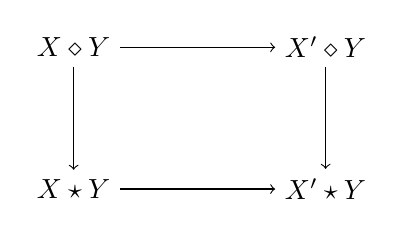
\begin{tikzpicture}
  \node (tl) at (0,0) {$X \diamond Y$};
  \node (tr) at (3.2,0) {$X' \diamond Y$};
  \node (bl) at (0,-1.8) {$X \star Y$};
  \node (br) at (3.2,-1.8) {$X' \star Y$};
  \draw[->] (tl) -- (tr);
  \draw[->] (tl) -- (bl);
  \draw[->] (tr) -- (br);
  \draw[->] (bl) -- (br);
\end{tikzpicture}
\end{center}
中，上面的水平映射由\cref{cor:fat-join-joyal-equivalence}是一个\trJoyalEquivalence{}，
而诸竖直映射由\cref{prop:fat-join-joyal-equivalence}是\trJoyalEquivalence{}。
\end{proof}

\begin{definition}\label{def:fat-slice}
设 $p\colon Y \to W$ 是 $\mathrm{sSet}_{Y/}$ 的一个\trObject{}。我们把 $p$ 的%
\emph{\trFatSlice{}}（fat slice）定义为\trSimplicialSet{} $W^{p/}$，由
\[
(W^{p/})_n = \mathrm{Hom}_{\mathrm{sSet}_{Y/}}(Y \diamond \Delta^n, W)
\]
给出，并把\trSimplicialSet{} $W^{/p}$ 定义为
\[
(W^{/p})_n = \mathrm{Hom}_{\mathrm{sSet}_{Y/}}(\Delta^n \diamond Y, W).
\]
\end{definition}

\begin{lemma}\label{lem:fat-slice-right-adjoint}
由把 $p\colon Y \to W$ 送到 $W^{/p}$ 所给出的\trFunctor{}%
$\mathrm{sSet}_{Y/} \to \mathrm{sSet}$ 是\trFunctor{} $- \diamond Y$ 的右伴随。
同样地，\trFunctor{} $p \mapsto W^{p/}$ 是\trFunctor{} $Y \diamond -$ 的右伴随。
\end{lemma}

\begin{proof}
按定义，伴随双射对可表示对象成立，从而对所有\trSimplicialSets{}成立，因为%
\trFunctor{} $- \diamond Y$ 与 $Y \diamond -$ 由\cref{lem:fat-join-colimit}保持
余极限。
\end{proof}

\begin{lemma}\label{lem:fat-slice-ordinary-map}
设 $Y$ 是一个\trSimplicialSet{}，而 $p\colon Y \to W$ 是\trSimplicialSets{}的一个
映射。那么存在典范映射 $W_{/p} \to W^{/p}$ 与 $W_{p/} \to W^{p/}$。
\end{lemma}

\begin{proof}
在 $n$-\trSimplex{}上，我们必须提供一个映射
\[
\mathrm{Hom}_{\mathrm{sSet}_{Y/}}(Y \star \Delta^n, W)
\longrightarrow
\mathrm{Hom}_{\mathrm{sSet}_{Y/}}(Y \diamond \Delta^n, W).
\]
为此，只需回忆起 $\mathrm{sSet}_{Y/}$ 中存在一个映射
$Y \diamond \Delta^n \to Y \star \Delta^n$，它对单形范畴 $\Delta$ 中的映射是自然的。对另一个\trSlice{}亦有同理。
\end{proof}

作为\cref{thm:isofibration-lifting-joyal-equivalence}的一个推论，我们可以对\trFatSlice{}%
建立第 1 章中的\cref{thm:slice-fibration}的一个类似物。

\begin{lemma}\label{lem:fat-slice-fibration}
设
\[
S \xrightarrow{\ i\ } T \xrightarrow{\ f\ } \C \xrightarrow{\ p\ } \D
\]
是\trSimplicialSets{}的一些映射，使得 $i$ 是一个\trMonomorphism{}，而 $p$ 是
∞-\trCategories{}之间的一个\trIsofibration{}。那么\trFunctor{}%
\[
\C^{f/} \longrightarrow \D^{pf/} \times_{\D^{pfi/}} \C^{fi/}
\]
是一个\trLeftFibration{}。同样地，\trFunctor{}%
\[
\C^{/f} \longrightarrow \D^{/pf} \times_{\D^{/pfi}} \C^{/fi}
\]
是一个\trRightFibration{}。
\end{lemma}

\begin{proof}
设 $A \to B$ 是一个\trLeftAnodyne{}映射，并考虑提升问题
\begin{center}
\begin{tikzpicture}
  \node (tl) at (0,0) {$A$};
  \node (tr) at (4.2,0) {$\C^{f/}$};
  \node (bl) at (0,-1.8) {$B$};
  \node (br) at (4.2,-1.8) {$\D^{pf/} \times_{\D^{pfi/}} \C^{fi/}$};
  \draw[->] (tl) -- (tr);
  \draw[->] (tl) -- (bl);
  \draw[->] (bl) -- (br);
  \draw[->] (tr) -- (br);
  \draw[->, dashed] (bl) -- (tr);
\end{tikzpicture}
\end{center}
由伴随性，这等价于提升问题
\begin{center}
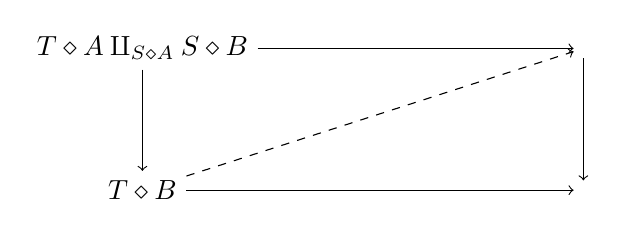
\begin{tikzpicture}
  \node (tl) at (0,0) {$T \diamond A \amalg_{S \diamond A} S \diamond B$};
  \node (tr) at (5.6,0) {$\C$};
  \node (bl) at (0,-1.8) {$T \diamond B$};
  \node (br) at (5.6,-1.8) {$\D$};
  \draw[->] (tl) -- (tr);
  \draw[->] (tl) -- (bl);
  \draw[->] (bl) -- (br);
  \draw[->] (tr) -- (br);
  \draw[->, dashed] (bl) -- (tr);
\end{tikzpicture}
\end{center}
其中左边的竖直映射是一个\trMonomorphism{}。我们想证明它是一个\trJoyalEquivalence{}，
从而可以援引\cref{thm:isofibration-lifting-joyal-equivalence}来结束本引理。为此，
我们断言：在图表
\begin{center}
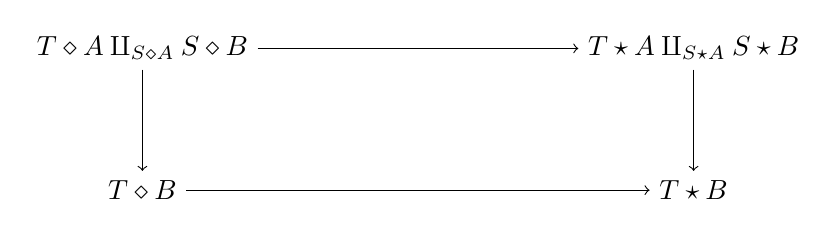
\begin{tikzpicture}
  \node (tl) at (0,0) {$T \diamond A \amalg_{S \diamond A} S \diamond B$};
  \node (tr) at (7.0,0) {$T \star A \amalg_{S \star A} S \star B$};
  \node (bl) at (0,-1.8) {$T \diamond B$};
  \node (br) at (7.0,-1.8) {$T \star B$};
  \draw[->] (tl) -- (tr);
  \draw[->] (tl) -- (bl);
  \draw[->] (tr) -- (br);
  \draw[->] (bl) -- (br);
\end{tikzpicture}
\end{center}
中，两个水平映射都是\trJoyalEquivalence{}：对下面的水平映射，这正是%
\cref{prop:fat-join-joyal-equivalence}；而对上面的水平映射，我们利用这些是沿%
\trMonomorphism{}的推出这一事实，于是对\cref{prop:fat-join-joyal-equivalence}作
三次应用并结合\cref{cor:pushout-joyal-equivalence}便证实了该断言。接下来，我们由第 1 章中的%
\cref{lem:join-box-anodyne}回忆起右边的竖直映射是\trInnerAnodyne{}的，从而是一个%
\trJoyalEquivalence{}。同样地，对另一个\trSlice{}的论证是一样的。
\end{proof}

\begin{remark}\label{rem:fat-slice-inner-fibration}
事实上，\cref{lem:fat-slice-fibration}的结论在更一般的情形下成立：若把 $p$ 换成
任意\trSimplicialSets{}之间的一个\trInnerFibration{}，结论仍成立，见
\cite[Theorem 1.2]{Ste18b}。
\end{remark}

\begin{corollary}\label{cor:fat-slice-infinity-category}
设 $p\colon Y \to \C$ 是一个图表，其中 $\C$ 是一个∞-\trCategory{}。那么\trFunctor{}%
$\C^{p/} \to \C$ 是一个\trLeftFibration{}，而\trFunctor{} $\C^{/p} \to \C$ 是一个%
\trRightFibration{}。特别地，$\C^{p/}$ 与 $\C^{/p}$ 都是∞-\trCategories{}。
\end{corollary}

\begin{proof}
这是\cref{lem:fat-slice-fibration}在特殊情形
$\varnothing \to Y \to \C \to \Delta^0$ 下的结果。
\end{proof}

\begin{proposition}\label{prop:slice-fat-slice-joyal-equivalence}
设 $p\colon Y \to \C$ 是一个图表。那么典范\trFunctor{}%
\[
\C_{p/} \longrightarrow \C^{p/}
\]
是一个\trJoyalEquivalence{}。对 $\C_{/p} \to \C^{/p}$ 亦有同样的结论。
\end{proposition}

\begin{proof}
我们只勾画一个证明。想法是证明：$X \star -$ 与 $X \diamond -$ 都是左\trQuillen{}%
\trFunctor{}，并且由\cref{prop:fat-join-joyal-equivalence}二者弱等价，从而在%
\trHomotopyCategory{}上诱导的\trFunctor{}同构。由此可得，相应的右伴随在%
\trHomotopyCategory{}中也同构，而这正是我们所需要的。对一个\trFunctor{}而言，是左%
\trQuillen{}\trFunctor{}意味着它保持\trMonomorphism{}，并且保持那些同时又是%
\trJoyalEquivalence{}的\trMonomorphism{}。对\trMonomorphism{}而言，这是显然的；
而对\trJoyalEquivalence{}，它由\cref{cor:join-joyal-equivalence}与%
\cref{cor:fat-join-joyal-equivalence}得出。因此，相应的右伴随保持\trTrivialFibration{}以及
∞-\trCategories{}之间的\trFibration{}。由此可得（证明正是在这里仍停留于梗概）：这两个\trSlice{}%
函子下降为\trJoyal{}\trModelStructure{}所关联的\trHomotopyCategory{}上那两个\trJoin{}函子的
右伴随。据此我们可以推出：\trSlice{}函子作为与那两个同构的\trJoin{}函子右伴随的函子，
也同构。
\end{proof}

借助通常\trSlice{}，我们也可以在∞-\trCategory{}中定义右映射空间与左映射空间。

\begin{definition}\label{def:left-right-mapping-space}
设 $\C$ 是一个∞-\trCategory{}，并设 $x$ 与 $y$ 是 $\C$ 的\trObject{}。我们把%
\emph{右\trMappingSpace{}}（right mapping space）定义为\trPullback{}%
\begin{center}
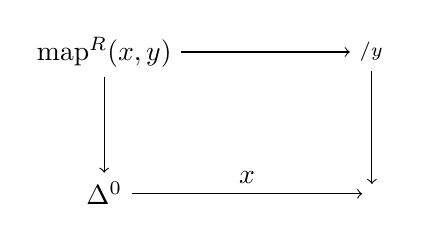
\begin{tikzpicture}
  \node (tl) at (0,0) {$\mathrm{map}^R_{\C}(x, y)$};
  \node (tr) at (3.4,0) {$\C_{/y}$};
  \node (bl) at (0,-1.8) {$\Delta^0$};
  \node (br) at (3.4,-1.8) {$\C$};
  \draw[->] (tl) -- (tr);
  \draw[->] (tl) -- (bl);
  \draw[->] (tr) -- (br);
  \draw[->] (bl) -- node[above] {$x$} (br);
\end{tikzpicture}
\end{center}
并把\emph{左\trMappingSpace{}}（left mapping space）定义为
\begin{center}
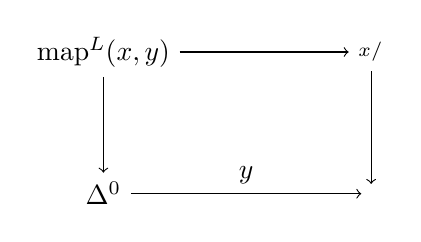
\begin{tikzpicture}
  \node (tl) at (0,0) {$\mathrm{map}^L_{\C}(x, y)$};
  \node (tr) at (3.4,0) {$\C_{x/}$};
  \node (bl) at (0,-1.8) {$\Delta^0$};
  \node (br) at (3.4,-1.8) {$\C$};
  \draw[->] (tl) -- (tr);
  \draw[->] (tl) -- (bl);
  \draw[->] (tr) -- (br);
  \draw[->] (bl) -- node[above] {$y$} (br);
\end{tikzpicture}
\end{center}
\end{definition}

\begin{remark}\label{rem:left-right-mapping-space-kan}
映射 $\mathrm{map}^R_{\C}(x, y) \to \Delta^0$ 是一个\trRightFibration{}，而映射
$\mathrm{map}^L_{\C}(x, y) \to \Delta^0$ 是一个\trLeftFibration{}。由\cref{ex:left-fibration-kan}，二者
实际上都是\trKanFibration{}，从而左、右\trMappingSpace{}都是\trKanComplex{}。
\end{remark}

接下来，我们想把这些映射空间与我们在第 1 章中的\cref{def:mapping-infinity-category}中已经定义
的\trMappingSpace{}相比较。下述引理将处理这件事。

\begin{lemma}\label{lem:slice-pullback}
下述两个图表都是\trPullback{}图表：
\begin{center}
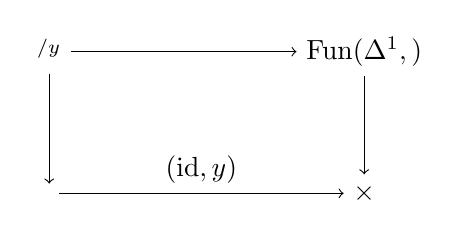
\begin{tikzpicture}
  \node (tl) at (0,0) {$\C^{/y}$};
  \node (tr) at (4.0,0) {$\mathrm{Fun}(\Delta^1, \C)$};
  \node (bl) at (0,-1.8) {$\C$};
  \node (br) at (4.0,-1.8) {$\C \times \C$};
  \draw[->] (tl) -- (tr);
  \draw[->] (tl) -- (bl);
  \draw[->] (tr) -- (br);
  \draw[->] (bl) -- node[above] {$(\mathrm{id}, y)$} (br);
\end{tikzpicture}
\hspace{1.6cm}
\begin{tikzpicture}
  \node (tl) at (0,0) {$\C^{x/}$};
  \node (tr) at (4.0,0) {$\mathrm{Fun}(\Delta^1, \C)$};
  \node (bl) at (0,-1.8) {$\C$};
  \node (br) at (4.0,-1.8) {$\C \times \C$};
  \draw[->] (tl) -- (tr);
  \draw[->] (tl) -- (bl);
  \draw[->] (tr) -- (br);
  \draw[->] (bl) -- node[above] {$(x, \mathrm{id})$} (br);
\end{tikzpicture}
\end{center}
\end{lemma}

\begin{proof}
我们只对左边的正方形给出证明。（对右边正方形的论证是类似的。）我们必须证明该图表
在所有 $n$-\trSimplex{}上是\trPullback{}，于是我们考虑如下图表：
\begin{center}
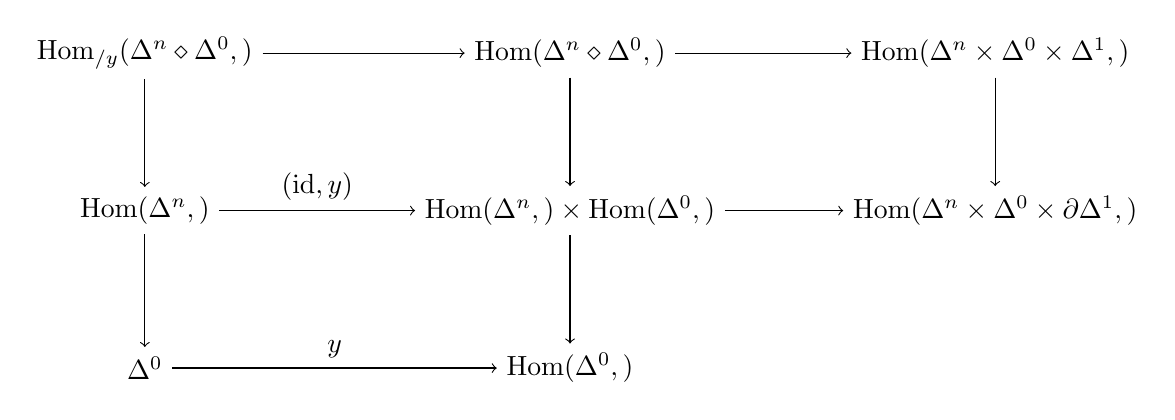
\begin{tikzpicture}
  \node (a) at (0,0)
    {$\mathrm{Hom}_{/y}(\Delta^n \diamond \Delta^0, \C)$};
  \node (b) at (5.4,0) {$\mathrm{Hom}(\Delta^n \diamond \Delta^0, \C)$};
  \node (c) at (10.8,0) {$\mathrm{Hom}(\Delta^n \times \Delta^0 \times \Delta^1, \C)$};
  \node (d) at (0,-2.0) {$\mathrm{Hom}(\Delta^n, \C)$};
  \node (e) at (5.4,-2.0)
    {$\mathrm{Hom}(\Delta^n, \C) \times \mathrm{Hom}(\Delta^0, \C)$};
  \node (f) at (10.8,-2.0)
    {$\mathrm{Hom}(\Delta^n \times \Delta^0 \times \partial\Delta^1, \C)$};
  \node (g) at (0,-4.0) {$\Delta^0$};
  \node (h) at (5.4,-4.0) {$\mathrm{Hom}(\Delta^0, \C)$};
  \draw[->] (a) -- (b);
  \draw[->] (b) -- (c);
  \draw[->] (a) -- (d);
  \draw[->] (b) -- (e);
  \draw[->] (c) -- (f);
  \draw[->] (d) -- node[above] {$(\mathrm{id}, y)$} (e);
  \draw[->] (e) -- (f);
  \draw[->] (d) -- (g);
  \draw[->] (g) -- node[above] {$y$} (h);
  \draw[->] (e) -- (h);
\end{tikzpicture}
\end{center}
为了证明上面的大正方形是\trPullback{}，首先注意，最右边的正方形由胖联
$\Delta^n \diamond \Delta^0$ 的定义本身是\trPullback{}。左下方的正方形经逐点检查
是\trPullback{}。左边两个正方形的组合按定义也是\trPullback{}。由此可知，左上方
的正方形是\trPullback{}。于是，把上面两个正方形组合起来，我们便得到所需的%
\trPullback{}。
\end{proof}

过渡到\trFibre{}，我们便得到下述推论。

\begin{corollary}\label{cor:mapping-space-pullback}
下述图表是\trPullback{}：
\begin{center}
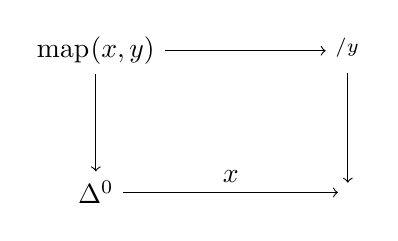
\begin{tikzpicture}
  \node (tl) at (0,0) {$\mathrm{map}_{\C}(x, y)$};
  \node (tr) at (3.2,0) {$\C^{/y}$};
  \node (bl) at (0,-1.8) {$\Delta^0$};
  \node (br) at (3.2,-1.8) {$\C$};
  \draw[->] (tl) -- (tr);
  \draw[->] (tl) -- (bl);
  \draw[->] (tr) -- (br);
  \draw[->] (bl) -- node[above] {$x$} (br);
\end{tikzpicture}
\hspace{1.6cm}
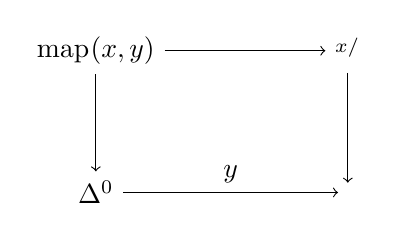
\begin{tikzpicture}
  \node (tl) at (0,0) {$\mathrm{map}_{\C}(x, y)$};
  \node (tr) at (3.2,0) {$\C^{x/}$};
  \node (bl) at (0,-1.8) {$\Delta^0$};
  \node (br) at (3.2,-1.8) {$\C$};
  \draw[->] (tl) -- (tr);
  \draw[->] (tl) -- (bl);
  \draw[->] (tr) -- (br);
  \draw[->] (bl) -- node[above] {$y$} (br);
\end{tikzpicture}
\end{center}
\end{corollary}

于是我们可以用下述引理来比较\trMappingSpace{}的种种定义。

\begin{lemma}\label{lem:isofibration-fibrewise}
考虑一个图表
\begin{center}
\begin{tikzpicture}
  \node (e) at (0,0) {$\E$};
  \node (e2) at (3.4,0) {$\E'$};
  \node (c) at (1.7,-1.8) {$\C$};
  \draw[->] (e) -- node[above] {$f$} (e2);
  \draw[->] (e) -- node[above left] {$p$} (c);
  \draw[->] (e2) -- node[above right] {$p'$} (c);
\end{tikzpicture}
\end{center}
其中 $p$ 与 $p'$ 是\trIsofibration{}，而 $f$ 是一个\trJoyalEquivalence{}。那么，对
$\C$ 中的所有\trObject{} $x$，在\trFibre{}上诱导的映射 $\E_x \to \E'_x$ 也是一个%
\trJoyalEquivalence{}。
\end{lemma}

\begin{proof}
这立即可由\cref{lem:pullback-joyal-equivalence}得出。
\end{proof}

\begin{remark}\label{rem:fibrewise-converse}
这个陈述的逆并不成立（也就是说，无法由 $f$ 逐\trFibre{}地是\trJoyalEquivalence{}推出
$f$ 是\trJoyalEquivalence{}，但见\cref{ex:inner-fibration-joyal-equivalence-fibrewise}）。不过，对\trLeftFibration{}与%
\trRightFibration{}这个陈述
是成立的（实际上，更一般地，对\trCocartesianFibration{}与\trCartesianFibration{}也成立，我们将在%
定理 3.1.27 中证明）。
\end{remark}

\begin{corollary}\label{cor:mapping-space-homotopy-equivalence}
设 $\C$ 是一个∞-\trCategory{}，并设 $x$ 与 $y$ 是 $\C$ 的\trObject{}。那么映射
\[
\mathrm{map}^R_{\C}(x, y) \longrightarrow \mathrm{map}_{\C}(x, y)
\longleftarrow \mathrm{map}^L_{\C}(x, y)
\]
都是\trHomotopyEquivalence{}。
\end{corollary}

\begin{proof}
把\cref{lem:isofibration-fibrewise}应用于图表
\begin{center}
\begin{tikzpicture}
  \node (a) at (0,0) {$\C_{/y}$};
  \node (b) at (3.4,0) {$\C^{/y}$};
  \node (c) at (1.7,-1.8) {$\C$};
  \draw[->] (a) -- (b);
  \draw[->] (a) -- (c);
  \draw[->] (b) -- (c);
\end{tikzpicture}
\hspace{1.6cm}
\begin{tikzpicture}
  \node (a) at (0,0) {$\C_{x/}$};
  \node (b) at (3.4,0) {$\C^{x/}$};
  \node (c) at (1.7,-1.8) {$\C$};
  \draw[->] (a) -- (b);
  \draw[->] (a) -- (c);
  \draw[->] (b) -- (c);
\end{tikzpicture}
\end{center}
并使用\cref{cor:fat-slice-infinity-category}与\cref{prop:slice-fat-slice-joyal-equivalence}。
\end{proof}

最后，我们想把 Kan-\trEnrichment{}范畴的\trCoherentNerve{}的映射空间，与该单纯范畴中现成的
映射 Kan 复形加以比较。这些证明超出了本书的范围，参见例如
\cite[Section 2.2.2]{Lur09}。下述定理的一个直接的组合式论证最近由\trHebestreit{}与%
\trKrause{}给出 \cite{HK20}。

\begin{theorem}\label{thm:coherent-nerve-mapping-space}
设 $\C$ 是一个 Kan-\trEnrichment{}范畴，并设 $x$ 与 $y$ 是 $\C$ 的\trObject{}。那么存在一个
典范映射
\[
\mathrm{Hom}_{\C}(x, y) \longrightarrow \mathrm{map}_{\mathrm{N}(\C)}(x, y),
\]
它是一个\trHomotopyEquivalence{}。这个映射的同伦类对 $x$ 与 $y$ 是自然的。
\end{theorem}

\begin{corollary}\label{cor:nerve-weak-equivalence}
设 $F\colon \C \to \C'$ 是 Kan-\trEnrichment{}范畴的一个\trWeakEquivalence{}。那么诱导的%
\trFunctor{} $\mathrm{N}(F)\colon \mathrm{N}(\C) \to \mathrm{N}(\C')$ 是∞-\trCategories{}的
一个\trJoyalEquivalence{}。
\end{corollary}

\begin{proof}
\trFunctor{} $\mathrm{N}(F)$ 是\trEssentiallySurjective{}，当且仅当 $F$ 在%
第 1 章中的\cref{def:weak-equivalence-simplicial}的意义下是\trWeaklyEssentiallySurjective{}。
此外，\cref{thm:coherent-nerve-mapping-space}表明，$F$ 是\trWeaklyFullyFaithful{}，
当且仅当 $\mathrm{N}(F)$ 是\trFullyFaithful{}。于是我们由%
\cref{thm:ffes-joyal-equivalence}结束证明。
\end{proof}

回忆，我们定义过单纯范畴 $\mathrm{CW}$，其\trObject{}是 \trCWComplex{}，而其映射的%
\trSimplicialSet{}由 $\mathcal{S}(\mathrm{map}(X, Y))$ 给出；它的\trCoherentNerve{}记作
$\mathrm{Spc}$。此外，我们定义过单纯范畴 $\mathrm{Kan}$，其\trObject{}是%
\trKanComplex{}，而其映射的\trSimplicialSet{}由内部 hom-集
$\underline{\mathrm{Hom}}(A, B)$ 给出。现在我们断言：存在一个按如下方式构造的%
\trFunctor{} $\mathrm{CW} \to \mathrm{Kan}$：在\trObject{}上，它把 $X$ 送到
$\mathcal{S}(X)$；在\trMorphism{}上，我们必须提供一个单纯映射
\[
\mathcal{S}(\mathrm{map}(X, Y)) \longrightarrow
\underline{\mathrm{Hom}}(\mathcal{S}(X), \mathcal{S}(Y)),
\]
它与合成相容。由伴随性，这等价于提供一个映射
\[
\mathcal{S}(\mathrm{map}(X, Y)) \times \mathcal{S}(X) \longrightarrow \mathcal{S}(Y).
\]
接下来，回忆 $\mathcal{S}$ 是一个右伴随，因而保持乘积。于是只需提供一个单纯映射
\[
\mathcal{S}(\mathrm{map}(X, Y) \times X) \longrightarrow \mathcal{S}(Y)
\]
其中我们可以使用通常的合成映射 $\mathrm{map}(X, Y) \times X \to Y$ 并应用%
\trFunctor{} $\mathcal{S}$。

\begin{corollary}\label{cor:spc-hat-joyal-equivalence}
前面所描述的\trFunctor{}%
$\mathrm{Spc} = \mathrm{N}(\mathrm{CW}) \to \mathrm{N}(\mathrm{Kan}) = \widehat{\mathrm{Spc}}$
是一个\trJoyalEquivalence{}。
\end{corollary}

\begin{proof}
我们来证明\trFunctor{} $\mathrm{CW} \to \mathrm{Kan}$ 是单纯\trCategories{}的一个%
\trWeakEquivalence{}。它是\trWeaklyEssentiallySurjective{}，因为每个\trKanComplex{} $X$
都\trHomotopyEquivalence{}于 $\mathcal{S}(|X|)$，从而（在等价的意义上）位于\trFunctor{}%
$\mathrm{CW} \to \mathrm{Kan}$ 的像之中。为了证明这个\trFunctor{}是\trFullyFaithful{}，我们必须
证明映射
\[
\mathcal{S}(\mathrm{map}(X, Y)) \longrightarrow
\underline{\mathrm{Hom}}(\mathcal{S}(X), \mathcal{S}(Y))
\]
是一个\trHomotopyEquivalence{}。而这成立，当且仅当复合
\[
\mathrm{map}(X, Y) \longrightarrow |\mathcal{S}(\mathrm{map}(X, Y))|
\longrightarrow |\underline{\mathrm{Hom}}(\mathcal{S}(X), \mathcal{S}(Y))|
\]
是一个\trHomotopyEquivalence{}。但对此，我们可以利用如下事实：对任何两个\trKanComplex{} $A$ 与
$B$，典范映射
\[
|\underline{\mathrm{Hom}}(A, B)| \longrightarrow \mathrm{map}(|A|, |B|)
\]
是一个\trHomotopyEquivalence{}。
\end{proof}

\begin{corollary}\label{cor:spc-fully-faithful}
典范\trFunctor{} $\mathrm{Spc} \to \mathrm{Cat}_{\infty}$ 是\trFullyFaithful{}。
\end{corollary}

\begin{proof}
这个\trFunctor{}由对单纯\trCategories{}的\trFunctor{}%
$\mathrm{Kan} \to \mathrm{Cat}^1_{\infty}$ 施加\trCoherentNerve{}而给出。因此，我们只需证明：对任何两个%
\trKanComplex{} $X$ 与 $Y$，典范映射
\[
\underline{\mathrm{Hom}}(X, Y) \longrightarrow \mathrm{Fun}(X, Y)^{\simeq}
\]
是一个\trHomotopyEquivalence{}。事实上，它是\trSimplicialSets{}之间的一个同构，于是本推论得证。
\end{proof}


